\section{Kinect Hardware}
Microsoft brachte im November 2010 mit dem Produkt Xbox Kinect eine neues Produkt auf den Markt. Mit diesem war es möglich, die Spielkonsole Xbox 360 über eine 3D-Kamera zu steuern und Spiele zu spielen. Das neuartige Kamera-Modul war nun erstmals ein preiswerter Sensor, um 3D-Bilddaten auszuwerten.
Im Folgenden wird auf die Hardware des Sensors näher eingegangen:\\[0.2cm]

\begin{figure}[H]						
	\centering							
	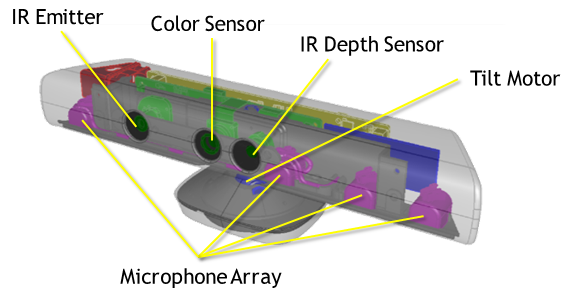
\includegraphics[scale=0.9]{Bilder/kinect_sensor_aufbau.png}			
	\caption{Aufbau Kinect\cite{ws:microsoft_kinect}}						
	\label{f:kinect_hardware}						
\end{figure}

\noindent
Das Kinectmodul besteht technisch gesehen aus mehreren Komponenten, die es ermöglichen, die
für diese Projektarbeit relevanten, abstrahierten Funktionen (Skelettverfolgung, Winkelextraktion, RGB-Bild)
zu realisieren. \cite{webb2012beginning}

\subsection{RGB-Kamera}

	Ein wesentlicher Teil der Kinect ist die RGB Kamera. Diese liefert ein Bild, das alleine
	oder auch in Kombinationen weiterer Funktionen verwendet werden kann.
	Das Sichtfeld der Kamera beträgt 43 Grad in der Vertikalen, sowie 57 Grad in der Horizontalen.
	Bei einer Auflösung von 640 x 480 Pixel werden 30 \ac{FPS} und bei 1280 x 960 Pixel noch 12 \ac{FPS} unterstützt.
	Wobei für viele Zwecke die geringere Auflösung genügt und deshalb auch standardmäßig verwendet wird \cite{jana2012kinect}.

\subsection{Tiefenerkennung}
	
	Der andere wesentliche Teil der Hardware besteht aus den Komponenten, die für die Tiefenerkennung
	zuständig sind. Diese Komponenten sind der \acf{IR-Emitter} und der IR-Tiefensensor (siehe	 Abb. 	 
	\ref{f:kinect_hardware}).\\
	\noindent
	Zur Abtastung der Tiefenwerte wendet die Kinect das \textit{Light-Coding} Prinzip an. Hierbei wird
	eine Szene mit einem Muster überlagert und daraus die Tiefeninformationen berechnet.
	Der \acs{IR-Emitter} sendet dabei ein spezielles Punktmuster aus (Siehe Abb. \ref{f:kinect_dots}),
	das vom Tiefensensor abgetastet werden kann.	
	
	\begin{figure}[H]						
		\centering							
		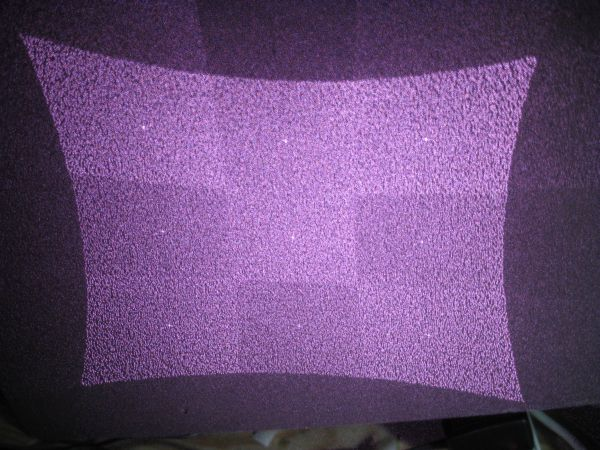
\includegraphics[scale=0.5]{Bilder/kinect_dots.jpg}			
		\caption{Kinect Punktemuster}						
		\label{f:kinect_dots}						
	\end{figure}
	
	\noindent	
	Der IR-Empfänger ist ein \acf{CMOS}-Chip und unterstützt eine maximale Auflösung
	von 640 x 480 Pixel.
	\\
	Die Einheit von Kinect, die für die Verarbeitung der Tiefen und RGB-Daten verantwortlich ist, ist
	der PrimeSense-Chip. Dieser wertet das Light-Coding mittels \textit{Depth from Focus} und 
	\textit{Depth from Stereo} aus.\cite{pdf:maccormick}
	\\
	Befindet sich nun ein Objekt im Sichtbereich der Kinect, wird das Muster auf das Objekt projiziert. Die räumliche Ausprägung des Objektes verzerrt dieses Muster (Siehe Abb. \ref{f:kinect_dots_with_Object}). Daraus kann der Chip die Tiefeninformationen errechnen.		
	
	
	\begin{figure}[H]						
		\centering							
		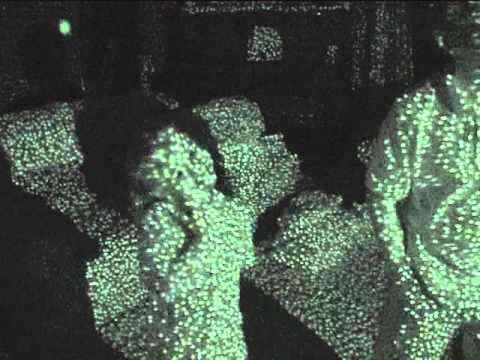
\includegraphics[scale=0.5]{Bilder/kinect_dots_green.jpg}			
		\caption{Kinect Objekte im Sichtraum}						
		\label{f:kinect_dots_with_Object}						
	\end{figure}
	
	\noindent
Die \textit{Depth from Focus} Methode beruht darauf, dass ein Gegenstand immer verschwommener wird, je weiter weg er sich von der Kinect befindet. Um diesen Effekt optimal zu nutzen, befindet sich vor dem Tiefensensor eine spezielle astigmatische Linse, die diesen Effekt zusätzlich verstärkt und einen Punkt zu einer Ellipse werden lässt, je weiter er von der Linse entfernt ist.\cite{pdf:maccormick}	\\
Die \textit{Depth from Stereo} Methode beruht auf der Parallaxe. Verändert ein Beobachter seine eigene Position, so beobachtet dieser eine scheinbare Änderung der Position des beobachteten Objektes \cite{pdf:parallaxe}. Hierbei erscheinen nahe liegende Objekte größer verschoben als weiter entfernte Objekte. Das "`Verschieben"' entsteht durch die Position der zwei Kameras. Anhand dieser Methoden kann der PrimeSense-Chip also die Tiefeninformationen aus der Szene extrahieren.	
	
Der Vorteil dieser Auswertung ist, dass zu einem Zeitpunkt nicht nur ein einzelner Punkt, sondern gleich eine komplette Punktewolke ausgerechnet und somit auch mehrere Bewegungen gleichzeitig erfasst werden können. Zum Beispiel eine Arm und eine Beinbewegung gleichzeitig. Zudem werden die Berechnung vom PrimeSense-Chip verarbeitet. Dies entlastet den angeschlossenen Computer.
	
	
\subsection{Tilt-Motor}
	Die Kinect besitzt einen Motor, um das Gehäuse in eine passende vertikale Position zu bringen.
	Der Kopf ist in vertikaler Richtung positiv, sowie negativ um 27 Grad verstellbar. Der Sensor kann
	dadurch optimal an die aktuelle Position angepasst werden, sodass eine Person im
	Kinectraum noch korrekt erkannt werden kann und sich innerhalb des Sichtfeldes befindet.
	\cite{jana2012kinect}
	
	
\subsection{Microphon Array}
	Die Hardware des Sensors enthält zusätzlich noch ein Mikrofonarray, das aus vier Mikrofonen besteht.
	Diese sind an der Vorderseite linear angeordnet. Drei befinden sich auf der rechten Seite und eines
	auf der linken Seite. Somit lässt sich die Richtung eines Geräusches identifizieren. Zusätzlich bietet
	diese Anordnung eine Möglichkeit Störgeräusche (Rauschen) aus einer Aufnahme zu entfernen und entstehende
	Echos zu unterdrücken. \\
	Es gibt auch eine Möglichkeit Sprachbefehle mit einer Grammatik aus der Kinect-Library zu extrahieren \cite{jana2012kinect}. Diese sind jedoch für 
	dieses Projekt irrelevant und so wird das Mikrofonarray nicht verwendet.
	
